\subsection{Sequence}
\label{sec:Sequence}
The purpose of the \sbol{Sequence} class is to represent the primary structure of a \sbol{Component} object and the manner in which it is encoded. This representation is accomplished  by means of the \sbol{elements} property and \sbol{encoding} property (\ref{uml:sequence}).

\begin{figure}[ht]
\begin{center}
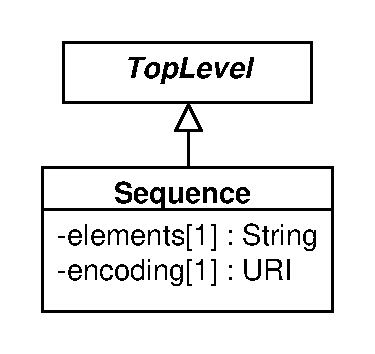
\includegraphics[scale=0.6]{uml/sequence}
\caption[]{Diagram of the \sbol{Sequence} class and its associated properties.}
\label{uml:sequence}
\end{center}
\end{figure}


\subparagraph{The \sbolheading{elements} property}
\label{sec:elements}
The \sbol{elements} property is an OPTIONAL \sbol{String} of characters that represents the constituents of a biological or chemical molecule. 
For example, these characters could represent the nucleotide bases of a molecule of DNA, the amino acid residues of a protein, or the atoms and chemical bonds of a small molecule.

If the \sbol{elements} property is not set, then it means the particulars of this \sbol{Sequence} have not yet been determined.

\subparagraph{The \sbolheading{encoding} property}
\label{sec:encoding}
The \sbol{encoding} property has a data type of \sbol{URI}, and is OPTIONAL unless \sbol{elements} is set, in which case it is REQUIRED.
This property MUST indicate how the \sbol{elements} property of a \sbol{Sequence} are formed and interpreted.

For example, the \sbol{elements} property of a \sbol{Sequence} with an IUPAC DNA encoding property MUST contain characters that represent nucleotide bases, such as {\tt a}, {\tt t}, {\tt c}, and {\tt g}. The \sbol{elements} property of a \sbol{Sequence} with a Simplified Molecular-Input Line-Entry System (SMILES) encoding, on the other hand, MUST contain characters that represent atoms and chemical bonds, such as {\tt C}, {\tt N}, {\tt O}, and {\tt =}.

\ref{tbl:sequence_encodings} provides a list of possible \sbol{URI} values for the \sbol{encoding} property. The terms in \ref{tbl:sequence_encodings} are organized by the type of \sbol{Component} (see \ref{tbl:component_types}) that typically refer to a \sbol{Sequence} with such an \sbol{encoding}. It is RECOMMENDED that the encoding property of a Sequence contains a URI from \ref{tbl:sequence_encodings}. When the \sbol{encoding} of a \sbol{Sequence} is well described by one of the \sbol{URI}s in \ref{tbl:sequence_encodings}, it MUST contain that \sbol{URI}.

More information on IUPAC encoding can be found at \url{http://www.bioinformatics.org/sms2/iupac.html}.

%A Summary of letters for nucleic acids and aminoacids
\begin{table}[ht]
  \begin{edtable}{tabular}{lll}
    \toprule
     \textbf{Encoding} & \textbf{URI} & \textbf{Component Type} \\
    \midrule
     IUPAC DNA, RNA & \url{http://sbols.org/v3#iupacNucleicAcid} & DNA, RNA \\
    IUPAC Protein & \url{http://sbols.org/v3#iupacAminoAcid} & Protein\\
   SMILES & \url{http://www.opensmiles.org/opensmiles.html} & Simple Chemical \\
    \bottomrule
  \end{edtable}
  \caption{\sbol{URI}s for specifying the \sbol{encoding} property of a \sbol{Sequence}, organized by the type of \sbol{Component} (see \ref{tbl:component_types}) that typically refer to a \sbol{Sequence} with such an \sbol{encoding}.}
  \label{tbl:sequence_encodings}
\end{table}
